\documentclass[12pt, a4paper]{extarticle}
\usepackage{geometry}
\geometry{
	a4paper,
	total={170mm,257mm},
	left=20mm,
	top=20mm,
	}
\usepackage{graphicx, float} % For figures
\usepackage{authblk}
\usepackage{amsmath}
\usepackage{amsmath, mathtools}
\usepackage{graphicx}
\usepackage{caption}
\usepackage{subcaption}
\usepackage{float}
\usepackage{wasysym}
\usepackage[procnames]{listings}
\usepackage{color}
\usepackage{multirow}
\usepackage{epstopdf}

%title and author details
\title{Aeroelastic Analysis of Hypersonic Double-wedge Lifting Surface}
\author[1]{Koorosh Gobal}
\author[1]{Anusha Anisetti}
\author[1]{(Vana Naga Samyuktha Nuthy )}
\affil[1]{Department of Mechanical and Materials Engineering, Wright State University}
\date{} %remove date

\begin{document}

\maketitle

\abstract{}
% ===================================================================
\section{Introduction}
{Nonlinear oscillations problem are important issues in physical science, mechanical structures and other engineering researches. Nonlinear systems display different behaviors than linear systems. They can exhibit
\begin{enumerate}  
\item  multiply steady state solutions, stable and unstable, in response to the same inputs (bifurcation),
\item  response at frequencies other than forcing frequency
\item  hysterisis with jump phenomenon, that includes discontinuous variations in the response of the system when system parameters are varied,
\item  irregular motions that are extremely sensitive to the initial conditions (chaos).
\end{enumerate}

Hence studying nonlinearieties is of extreme importance. As most of the real systems are modeled with non-linear differential equations, solving them is a critical task. There are many approximation methods to determine steady state solution in time domain. The drawback of such time-domain methods is the excessive need for computational time and resources. This can become a major bottle neck in design space exploration efforts of such systems where mutiple solutions
for different confgurations is needed. However, simulation in frequency domain eases the problem by transforming differential equations into algebraic complex equations and reduces the simulation cost by orders of magnitude. One such frequency domain approach to find steady state solution is the Harmonic Balance (HB) method.
\subsection{Harmonic Balance Method}
{Harmonic Balance Method assumes a truncated Fourier series as the solution to a nonlinear system. 
\begin{equation}
x(t) = a_0+\sum\limits_{n=1}^N (a_n \cos(n\omega t)+b_n \sin(n \omega t))
\end{equation}

where $\omega$ is the angular frequency with time period $T$ of the solution and $N$ is the order of truncation. 
The assumed solution is substituted into the equation of motion to determine the fourier coefficients to form an approximate closed form solution. The high-order harmonic components contribute significantly to whole solution for accuracy, where as a truncated series expantion makes the solution less accurate. If more harmonics are included, it becomes quite complext to solve the algebraic expressions for the Fourier coefficients.

\subsubsection{Advantages}
\begin{itemize}
\item{For some equations, a first-order truncated Fourier series can provide accurate results, especially as measure in terms of percentage error for the angular frequency $\omega$}
\item{Provides a close to accurate solution to steady-state responses.}
\end{itemize}

\subsubsection{Disdvantages}
\begin{itemize}
\item{Harmonic balance procedure cannot be applied to non-conservative oscillators as such systems involve transient behaviors}
\item{Determining the angular frequency and amplitudes may become algebraically complext.}
\end{itemize}

In this report, Harmonic balance methodology is first adapted on  linear equations and then extended to basic non-linear equations with closed form solution for comparison and extended to non-linear equations of first and second order. The results are compared with time integrated solutions of the corresponding systems.}

In this report, Harmonic balance methodology is first build on closed form equation for structural response of linear equations and then extended to basic non-linear equations and non-linear equations with parametric excitations. The results are compared with time integrated solutions of the corresponding systems.}

% ===================================================================
\section{Numerical Approach}

\begin{figure}[h]
	\centering
	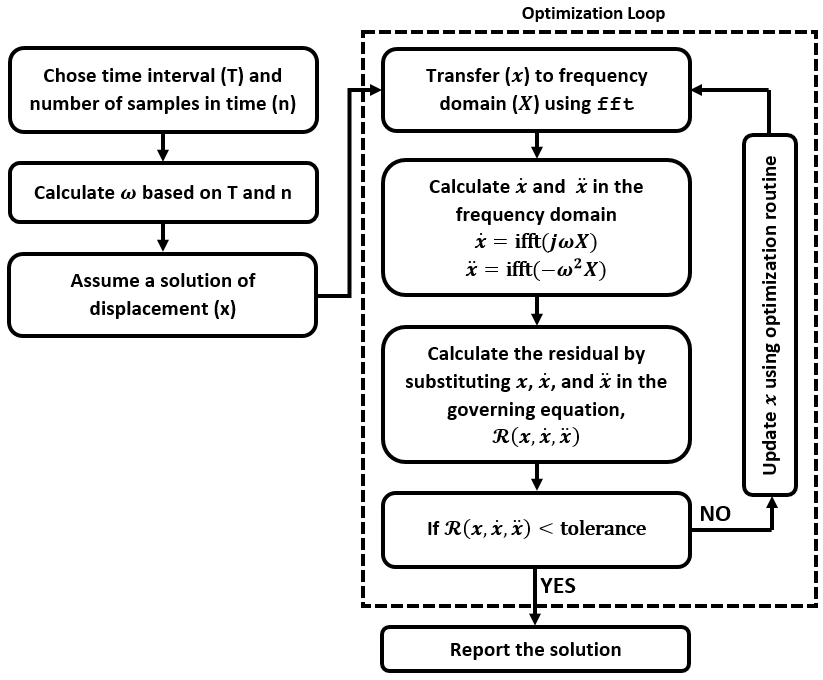
\includegraphics[height=9.00cm]{figure/minimize_residual.png}
	\caption{Flowchart for numerical approach.}
	\label{fig:flowchart}
\end{figure}

% ===================================================================
\section{Demonstration Results}
In this section, we apply the method of harmonic balance to different linear and non-linear problems. For the cases where analytical results are not available, we use numerical time integration to verify the results where it shows a good comparison. It should be noted that since the harmonic balance method is used to calculate the limit cycle oscillations of the system. Therefore, it is needed to let the transient part of time integration to die out. Only after this point, the two results match.

% -------------------------------------------------------------------
\subsection{Linear MCK System}
For the first demonstration case we looked at the forced linear damped oscillation of a single degree of freedom system. The governing equation is defined in Equation \eqref{eq:1GE}

\begin{equation}\label{eq:1GE}
	\ddot{x} + \dot{x} + x = \sin 2t
\end{equation}

This equation has a closed form solution that we can use to verify the harmonic balance result. The solution for Equation \eqref{eq:1GE} is calculated as

\begin{equation}
	x(t) = -0.23 \sin 2t - 0.15 \cos 2t
\end{equation}

The comparison between the HB and analytical result for Equation \eqref{eq:1GE} is shown in Figure \ref{fig:R1} for different number of harmonics in HB method. As can be seen here, the HB results matches perfectly with analytical solution of the system.

\begin{figure}[H]
	\centering
	\begin{subfigure}[h]{8.0 cm}
		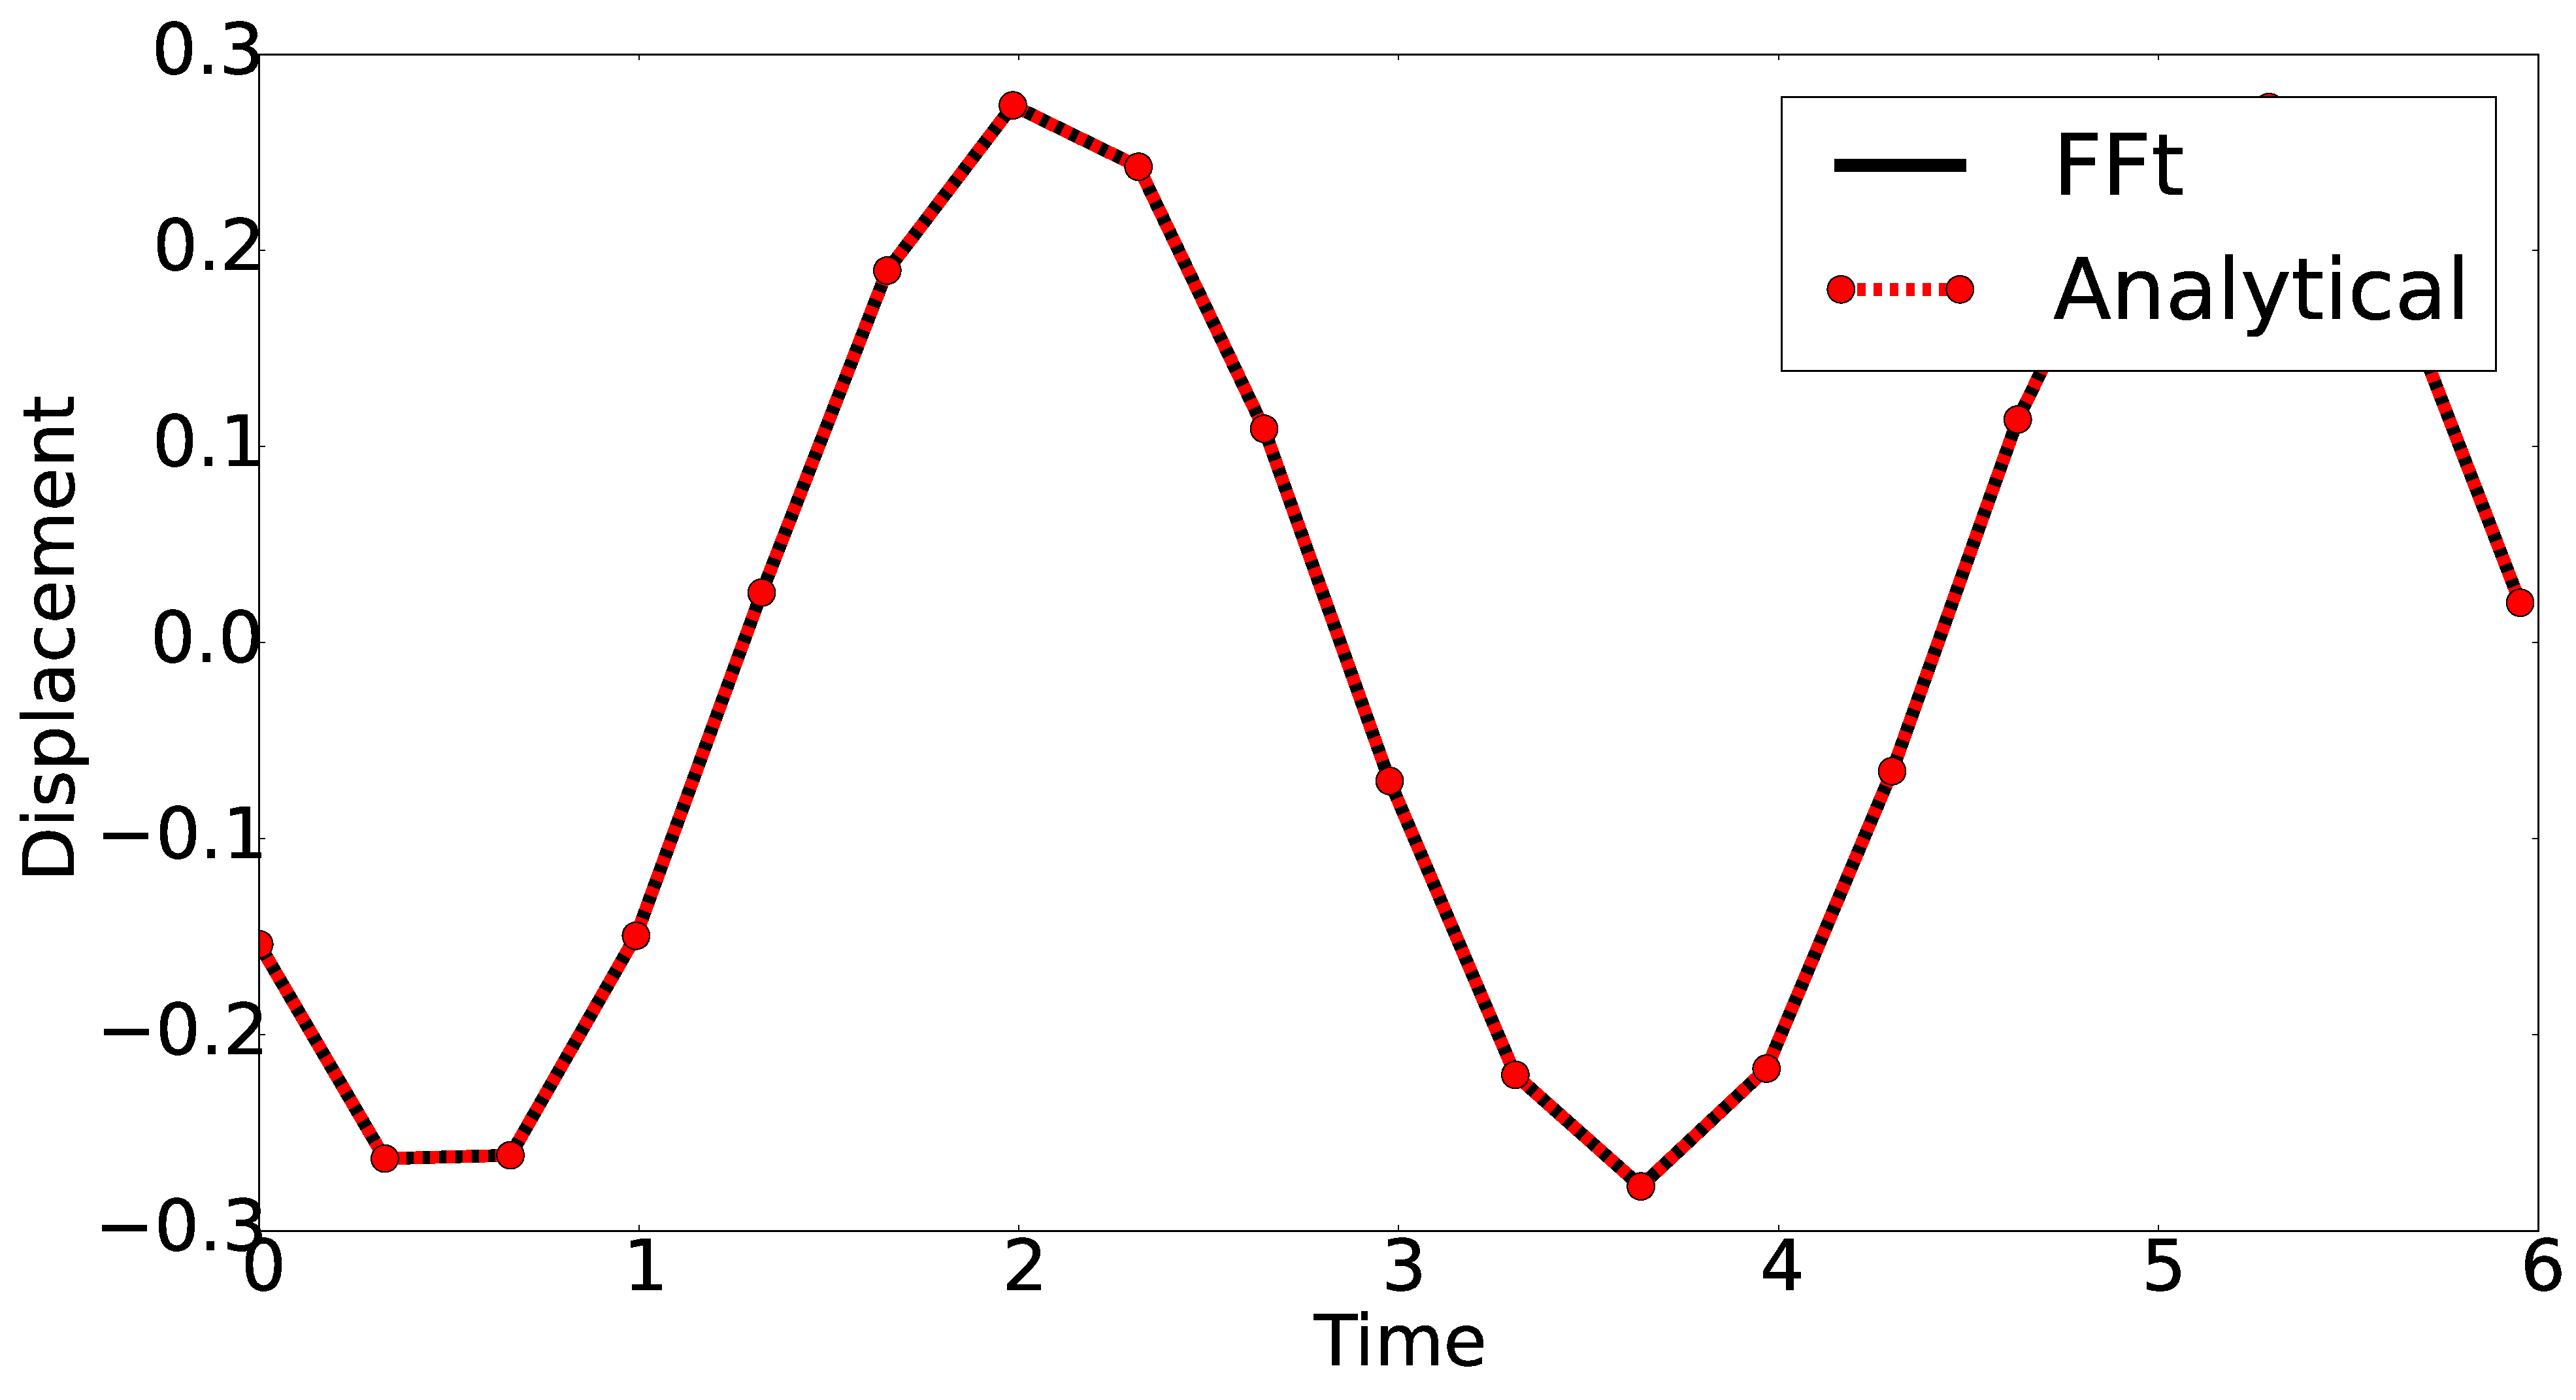
\includegraphics[width=8.0 cm]{figure/1N19.eps}
		\caption{n = 19}
	\end{subfigure}
	\begin{subfigure}[h]{8.0 cm}
        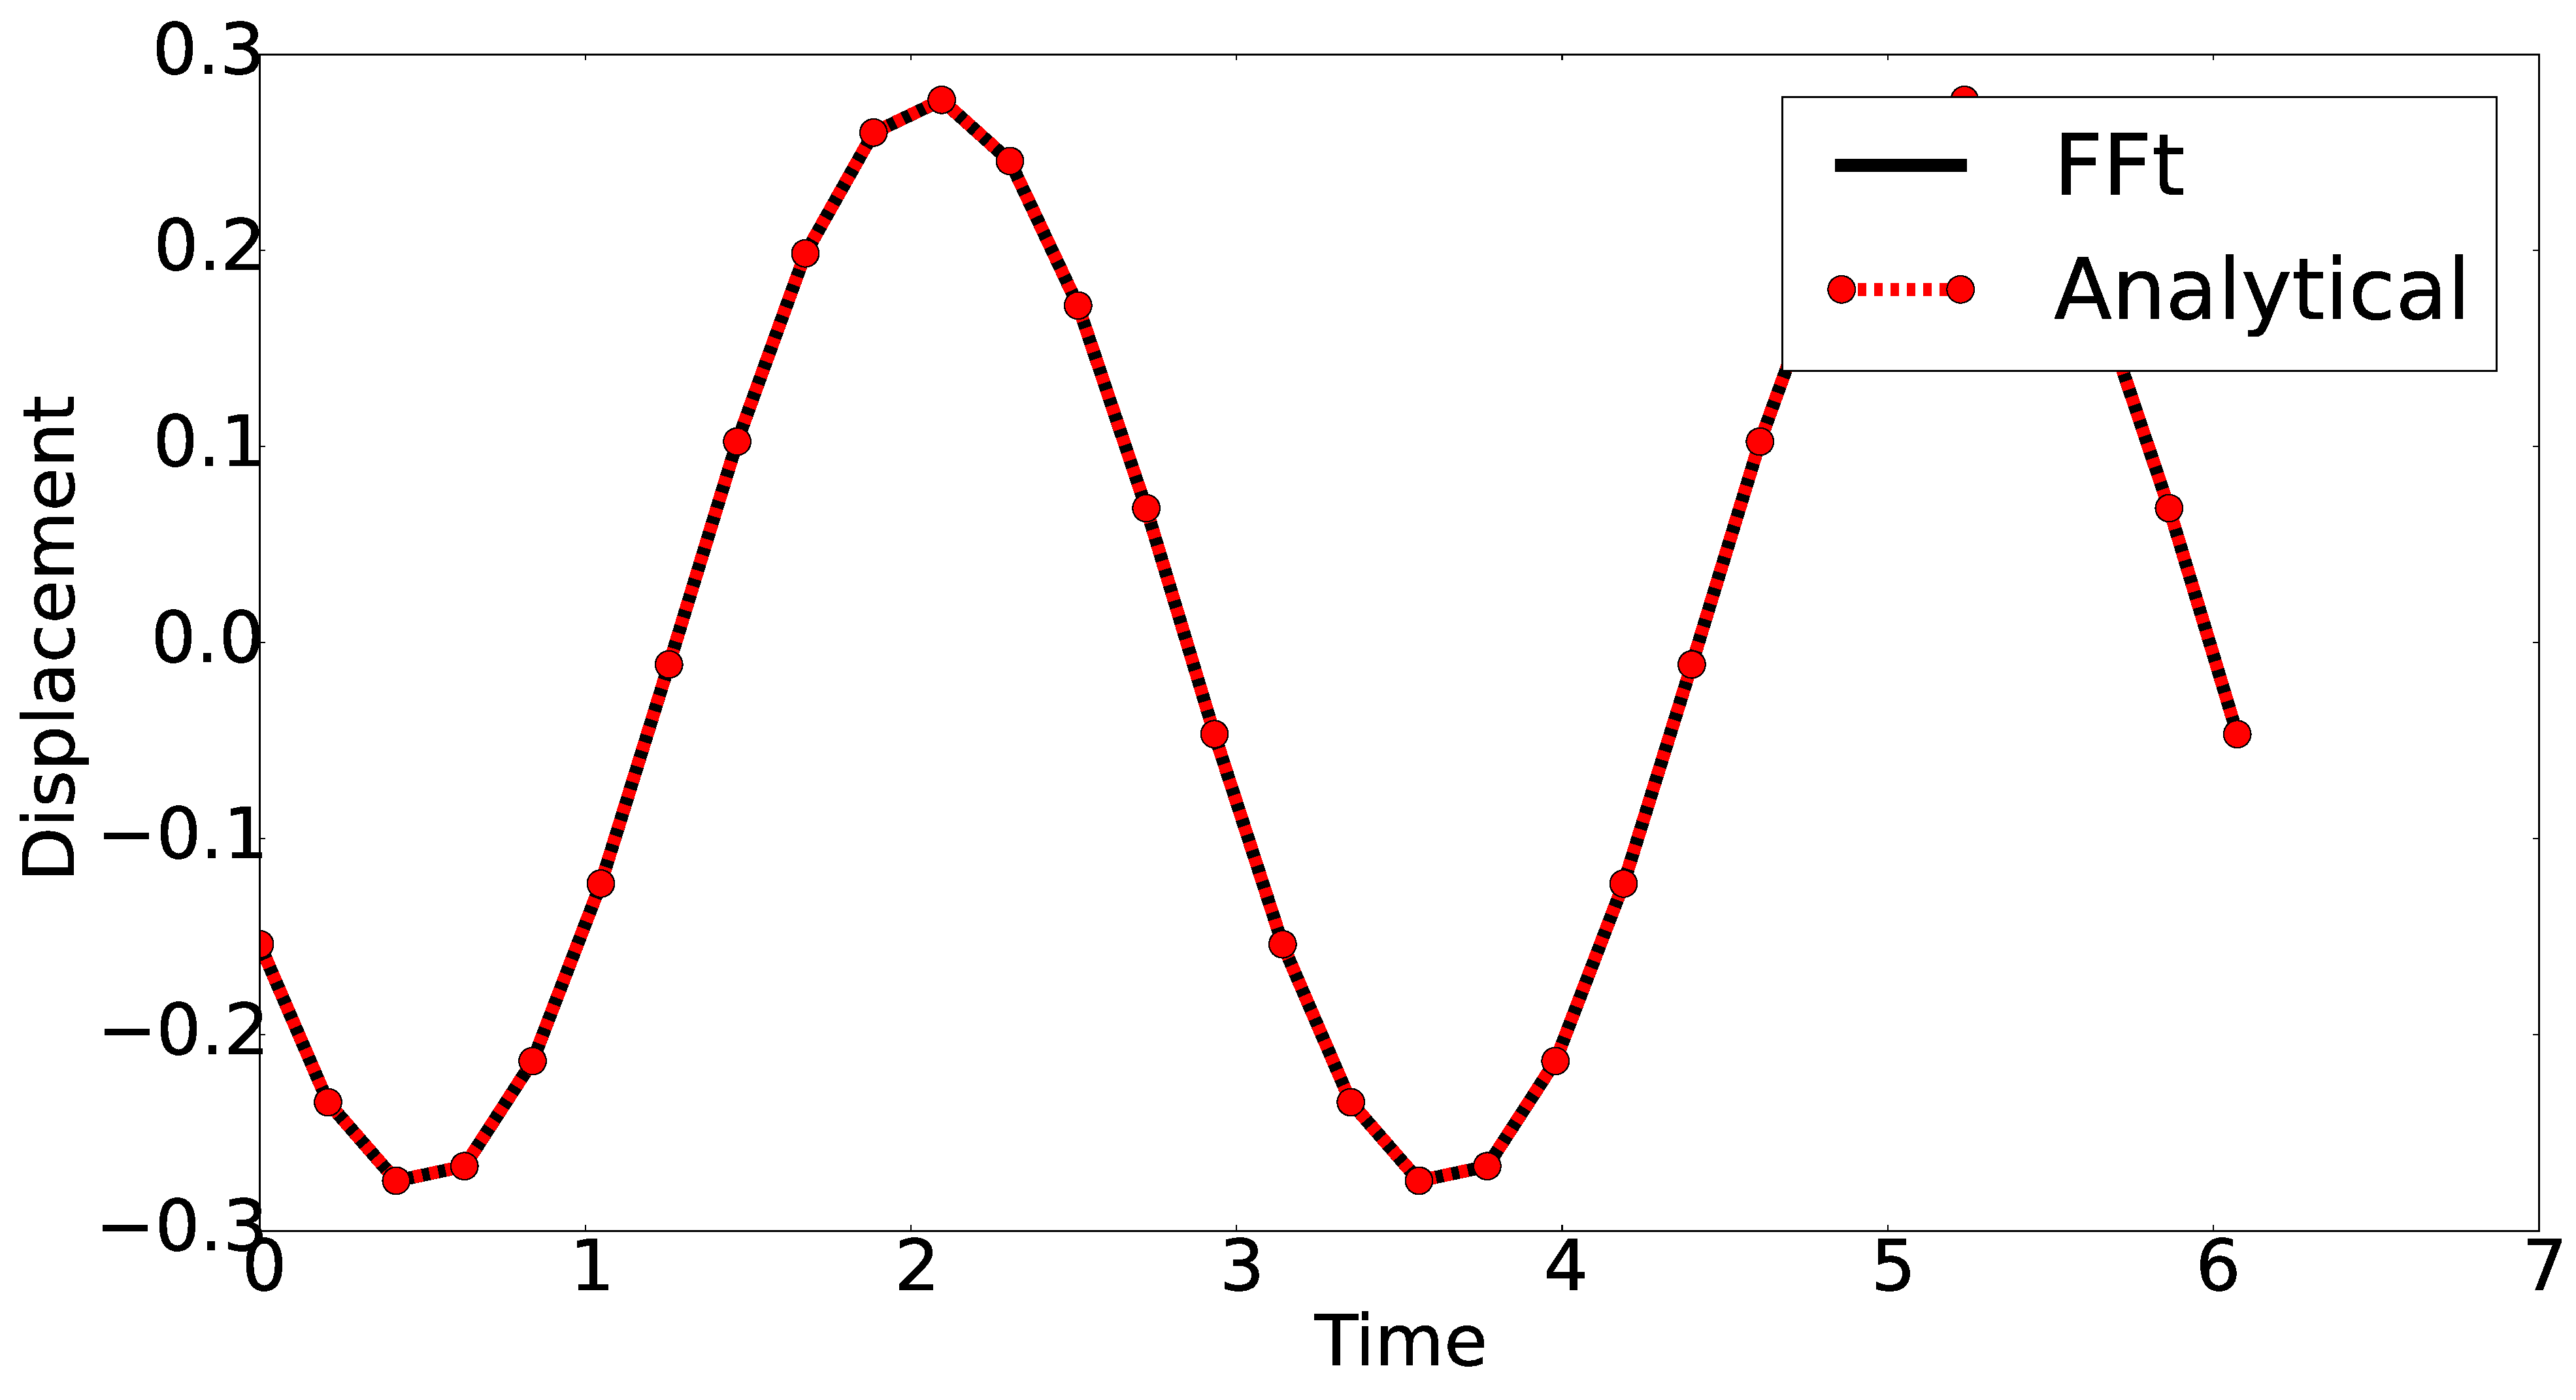
\includegraphics[width=8.0 cm]{figure/1N30.eps}
		\caption{n = 30}
    \end{subfigure}
    \caption{Comparison between HB and analytical result.}
    \label{fig:R1}
\end{figure}
% -------------------------------------------------------------------

\subsection{Linear System}
The governing equation is defined as
\begin{equation}\label{eq:samGE}
	\ddot{x} + x = \sin 2t
\end{equation}
 
The solution obtained from this equation can be used to compare with  the harmonic balance result. The solution for Equation \eqref{eq:samGE} is calculated as

\begin{equation}
	x(t) = -0.33 \sin 2t
\end{equation}

The following figure\ref{fig:samR1} shows the comparison results between the Harmonic Balance Method and analytical result for Equation \eqref{eq:samGE}. As it can be clearly seen, the Harmonic Balance Method results meets absolutely with analytical solution of the system.

\begin{figure}[H]
	\centering
	\includegraphics[width=8.0 cm]{figure/fig1.eps}
    \caption{Comparison between HB and analytical result.}
    \label{fig:samR1}
\end{figure}
% -------------------------------------------------------------------
\subsection{Nonlinear Oscillator}
For the second demonstration example, we looked at problem 2.45 on page 140 of Applied Nonlinear Dynamics (Nayfeh) book. The governing equation for this problem is shown in Equation \eqref{eq:2GE}

\begin{equation}\label{eq:2GE}
	\ddot{x} + 2 \mu \dot{x} + \frac{g}{R} \sin x - \alpha^2 \sin x \cos x = \sin 2t
\end{equation}

In above equation, we chose $\mu = 0.1$, $g = 9.81$, $R = 1.0$, and $\alpha = 1$. We used \texttt{odeint} function in \texttt{python} for time integration to verify the results of HB method. This is shown in Figure \ref{fig:R2}. As shown here, HB is in good agreement with the numerical solution at both low and high order sampling. The response converges and coincides with analytical solution as the transient part of the solution dies out.

\begin{figure}[H]
	\centering
	\begin{subfigure}[h]{8.0 cm}
		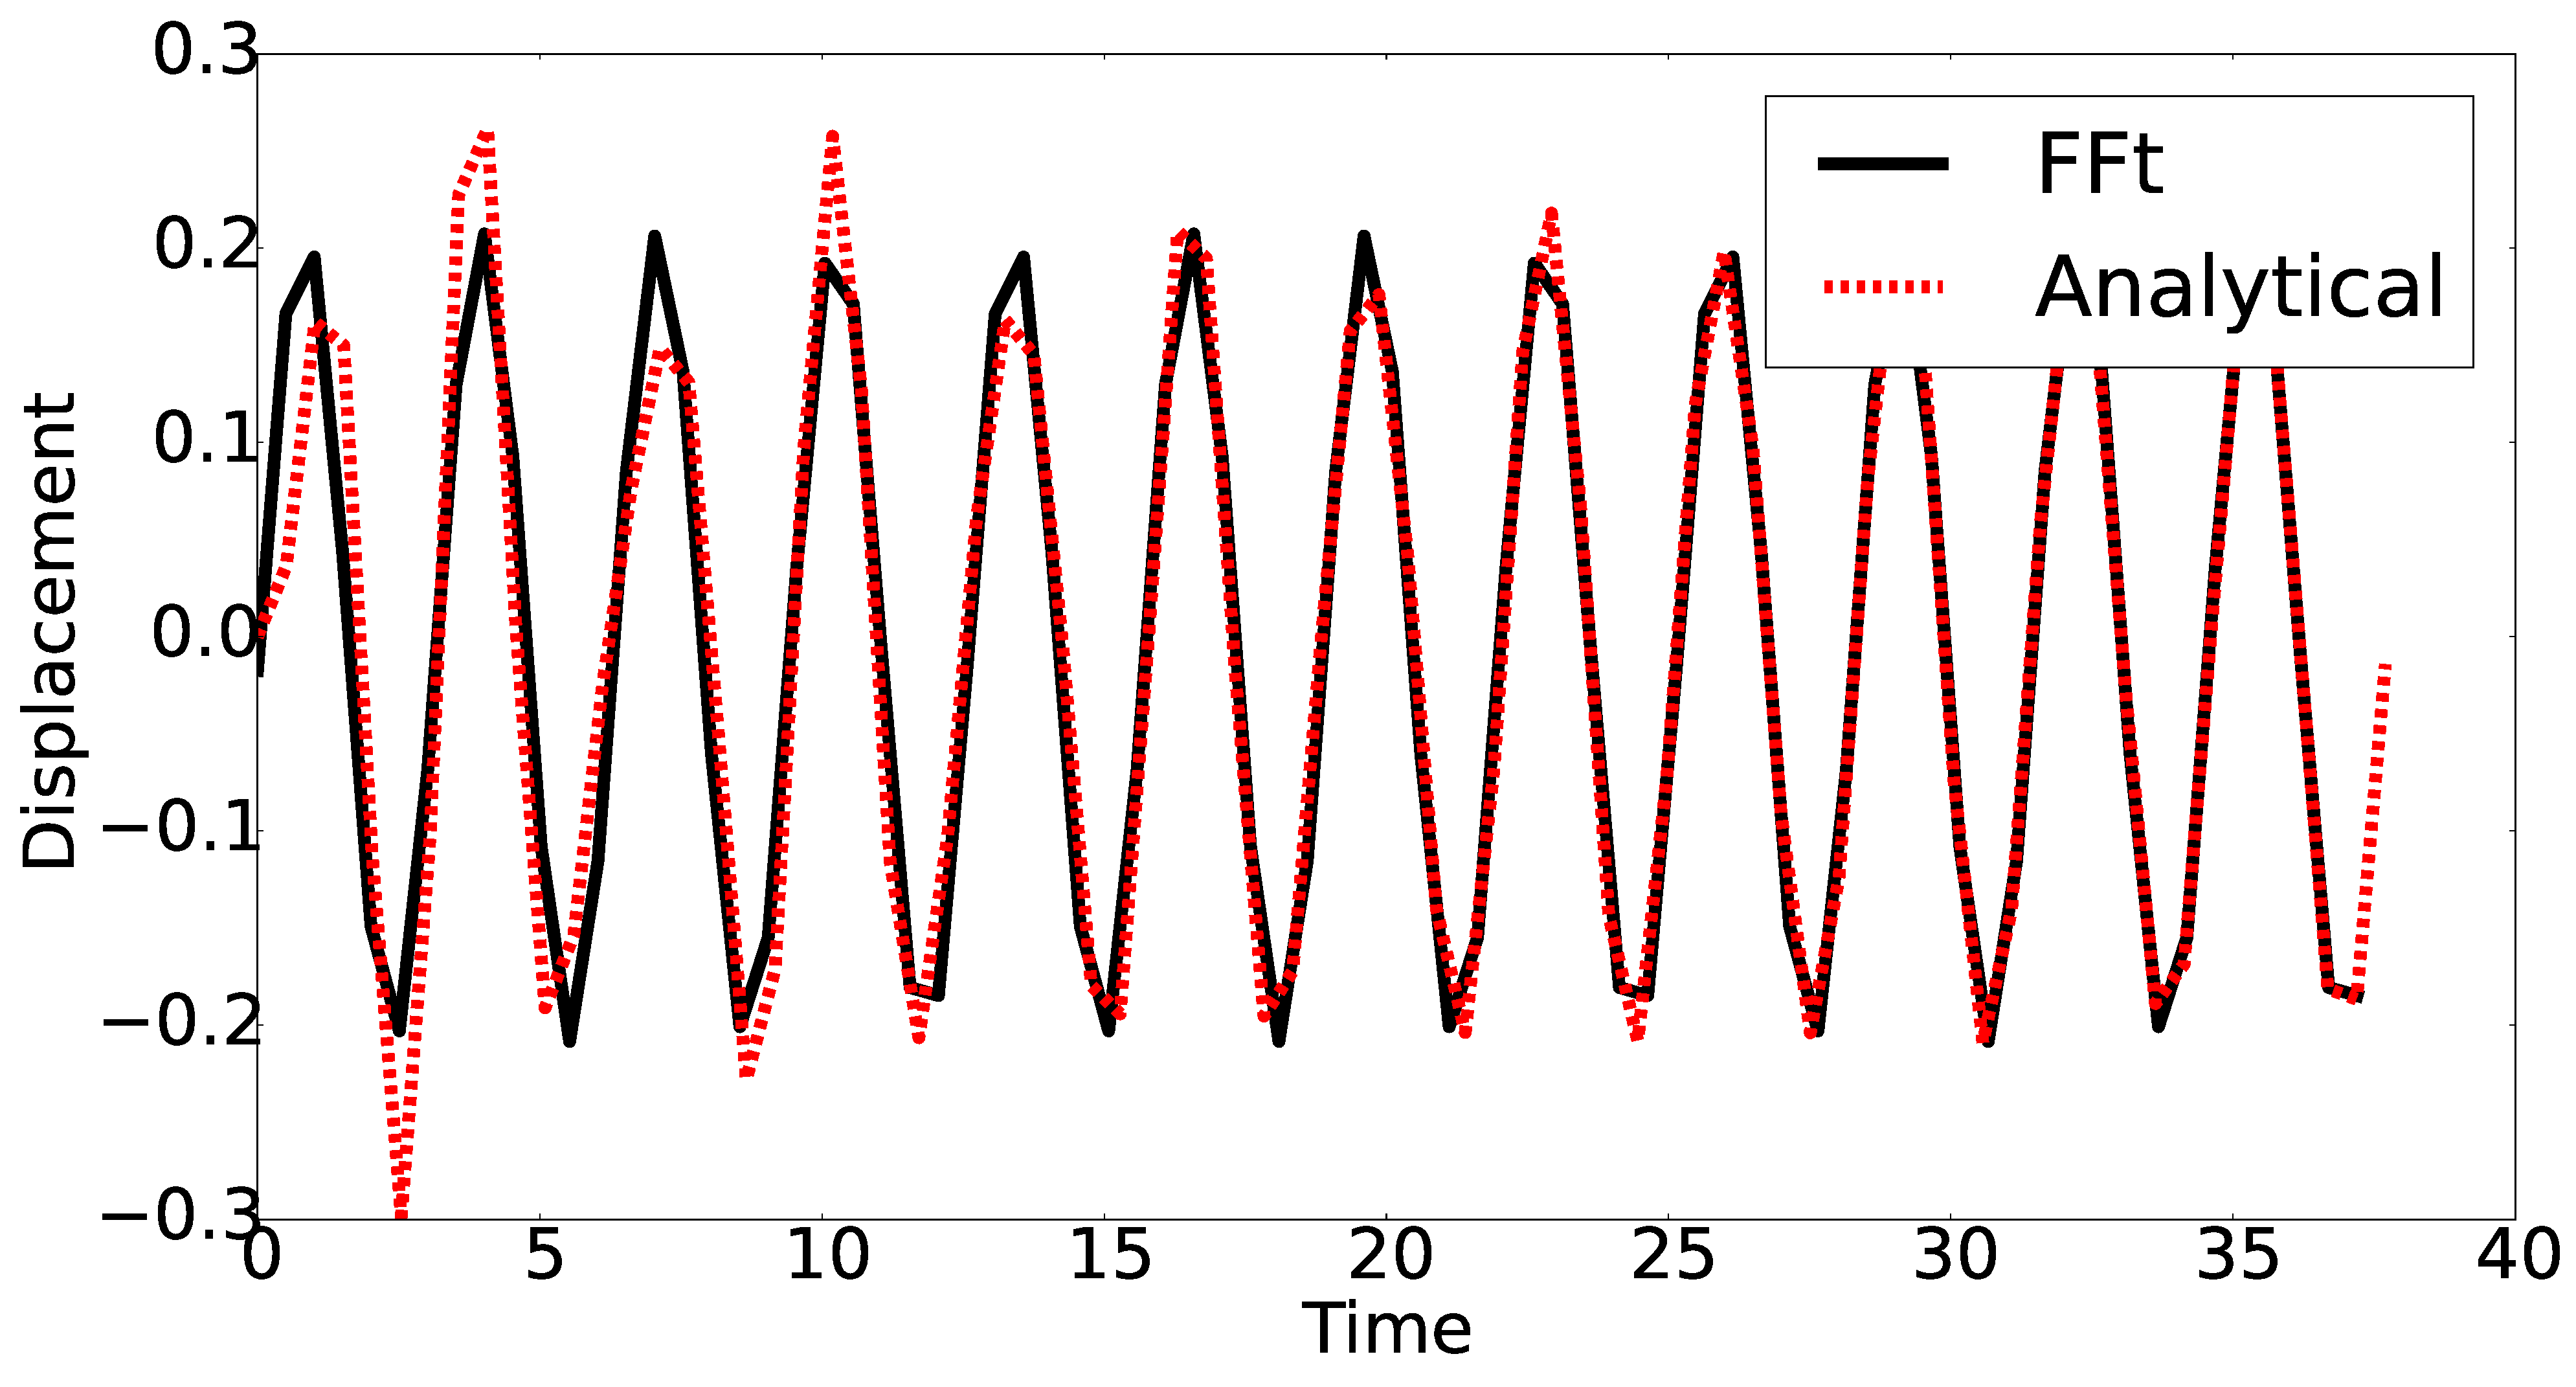
\includegraphics[width=8.0 cm]{figure/2N75.eps}
		\caption{n = 75}
	\end{subfigure}
	\begin{subfigure}[h]{8.0 cm}
        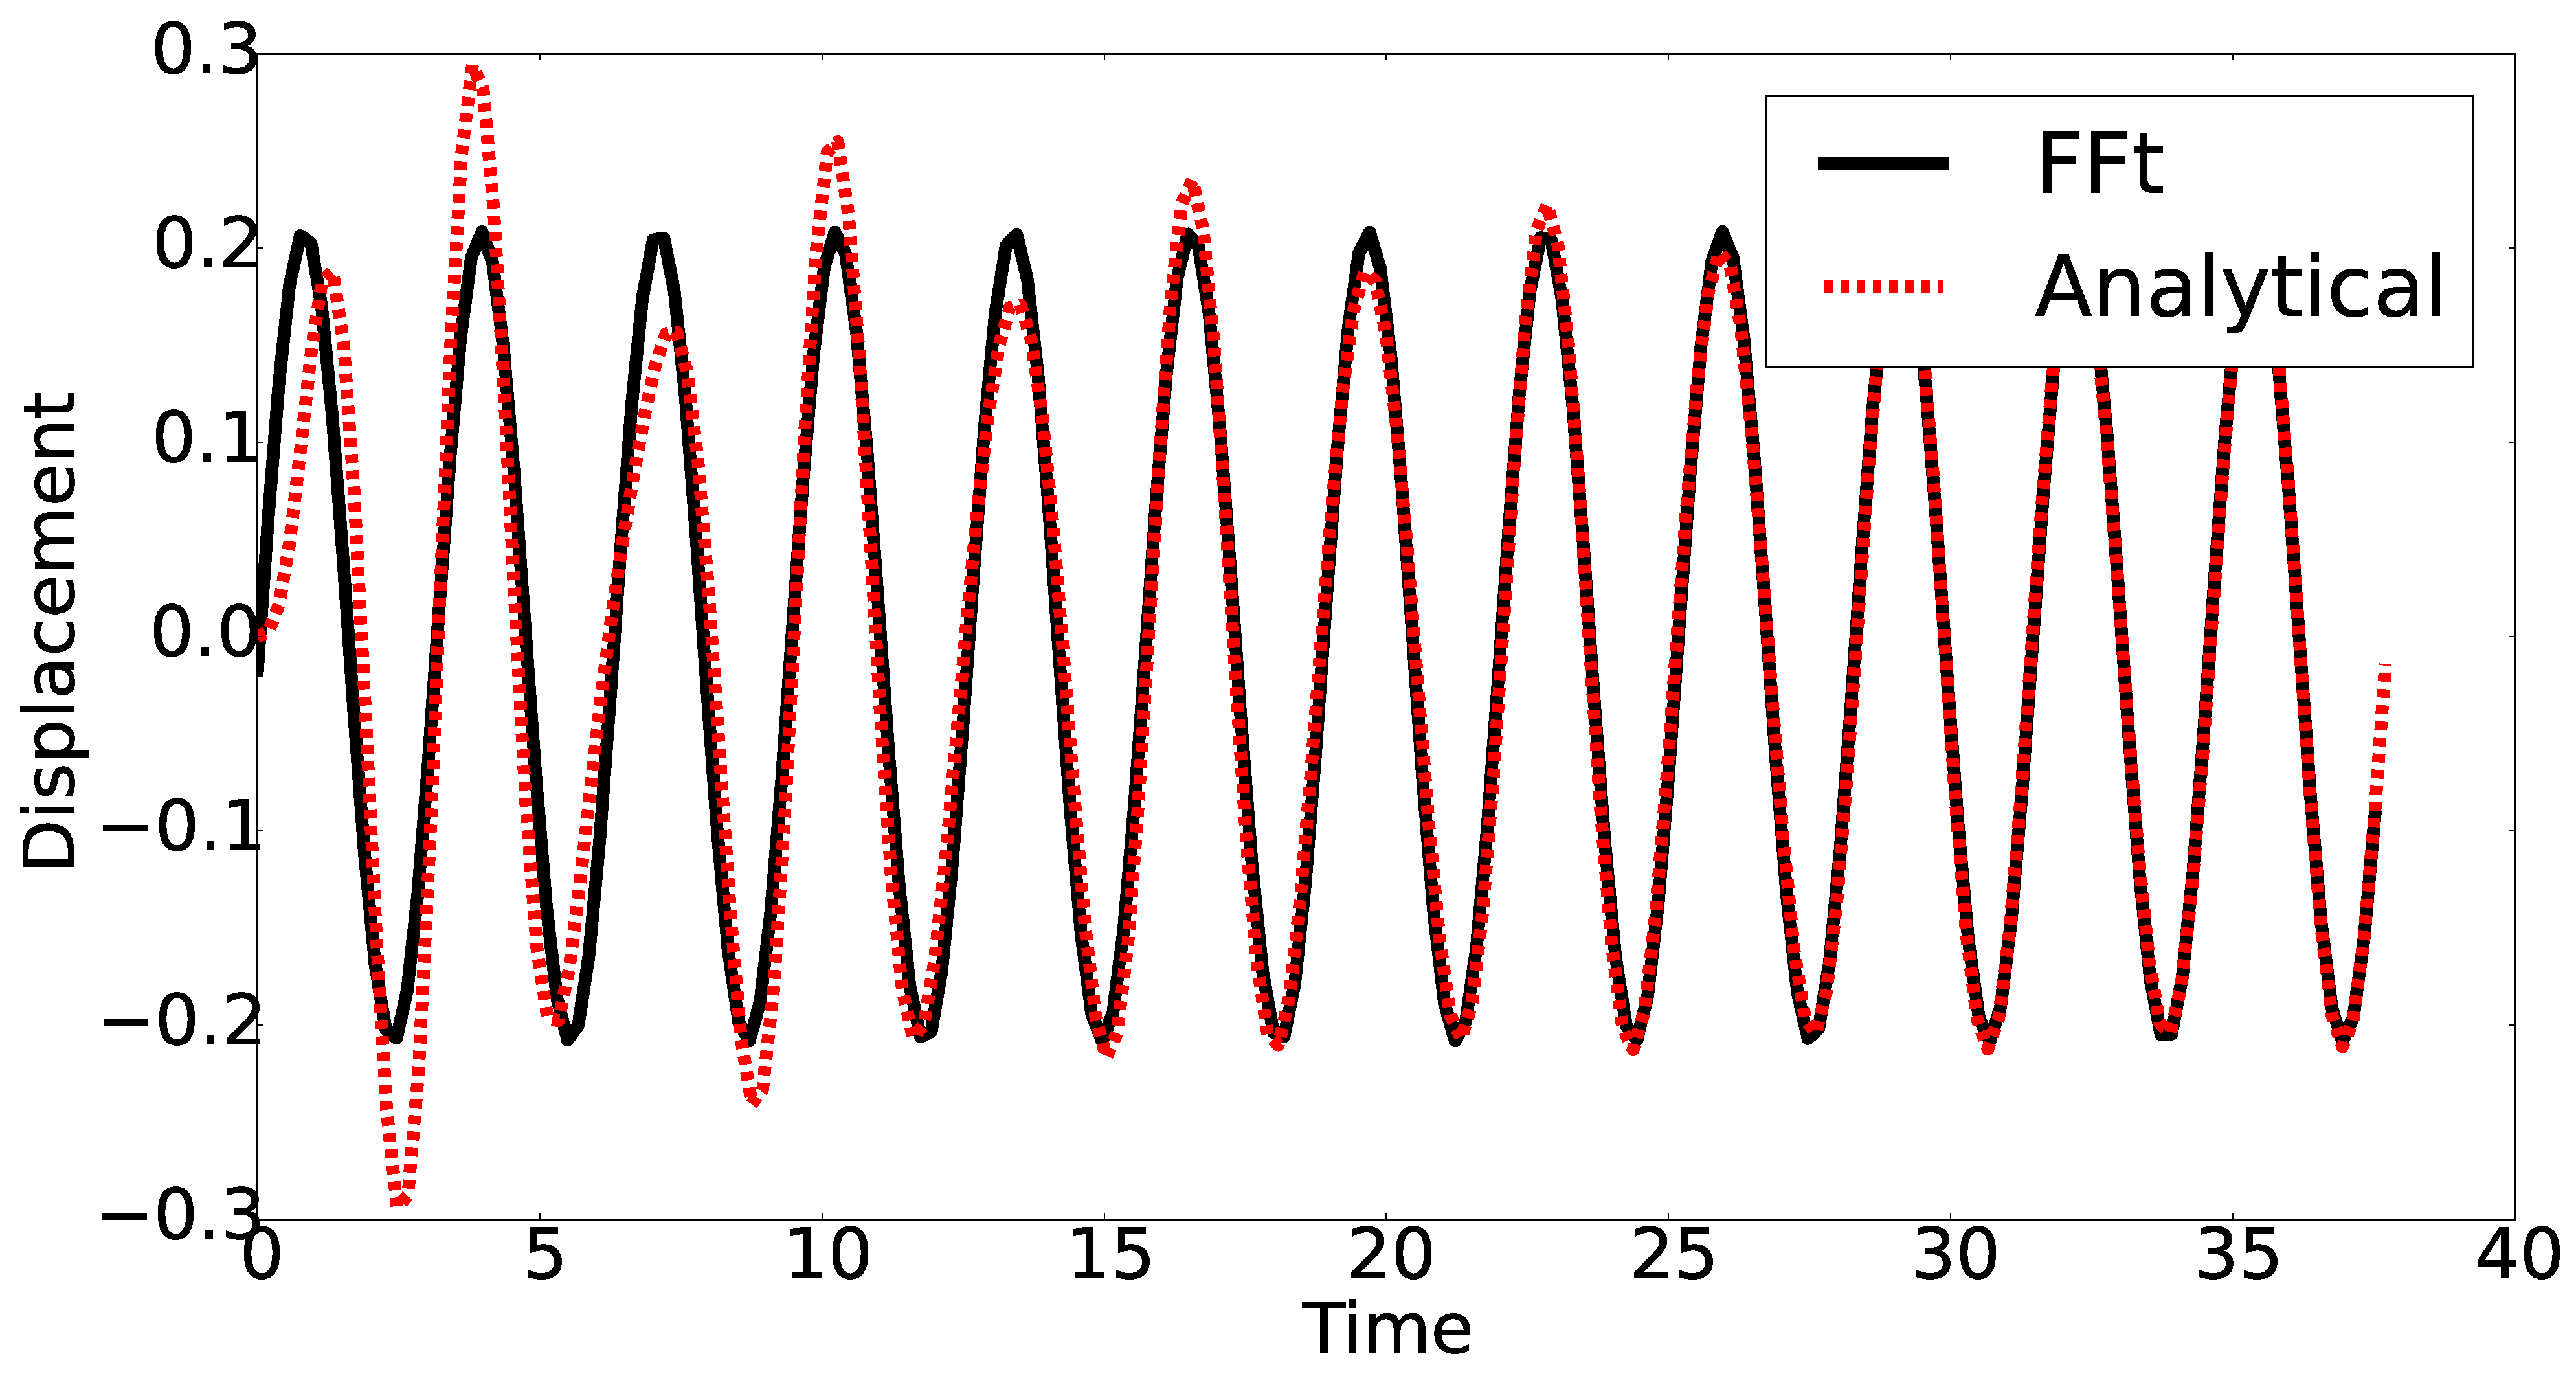
\includegraphics[width=8.0 cm]{figure/2N199.eps}
		\caption{n = 199}
    \end{subfigure}
    \caption{Comparison between HB and analytical result.}
    \label{fig:R2}
\end{figure}

% -------------------------------------------------------------------
\subsection{Parametrically excited Duffing Oscillator}
We looked at the applicability of HB in handling the nonlinear, force, parametrically excited Duffing oscillator. The governing equation of this system is shown in Equation \eqref{eq:3GE}.

\begin{equation}\label{eq:3GE}
	\ddot{x} + x + \epsilon \left[ 2 \mu \dot{x} + \alpha x^3 + 2 k x \cos \omega t \right] = \sin 2t	
\end{equation}

We chose $\epsilon = 1.0$, $\mu = 1.0$, $\alpha = 1.0$, $k = 1.0$, and $\omega = 2.0$ for the system parameters. Like the previous example, we used time integration to verify the results of HB method as shown in Figure \ref{fig:R3}. As seen here, similar convergence trend is observed for parametrically excited nonlinear oscillating system for different number of harmonics.

\begin{figure}[H]
	\centering
	\begin{subfigure}[h]{8.0 cm}
		
\includegraphics[width=8.0 cm]{figure/3N20.eps}
		\caption{n = 20}
	\end{subfigure}
	\begin{subfigure}[h]{8.0 cm}
        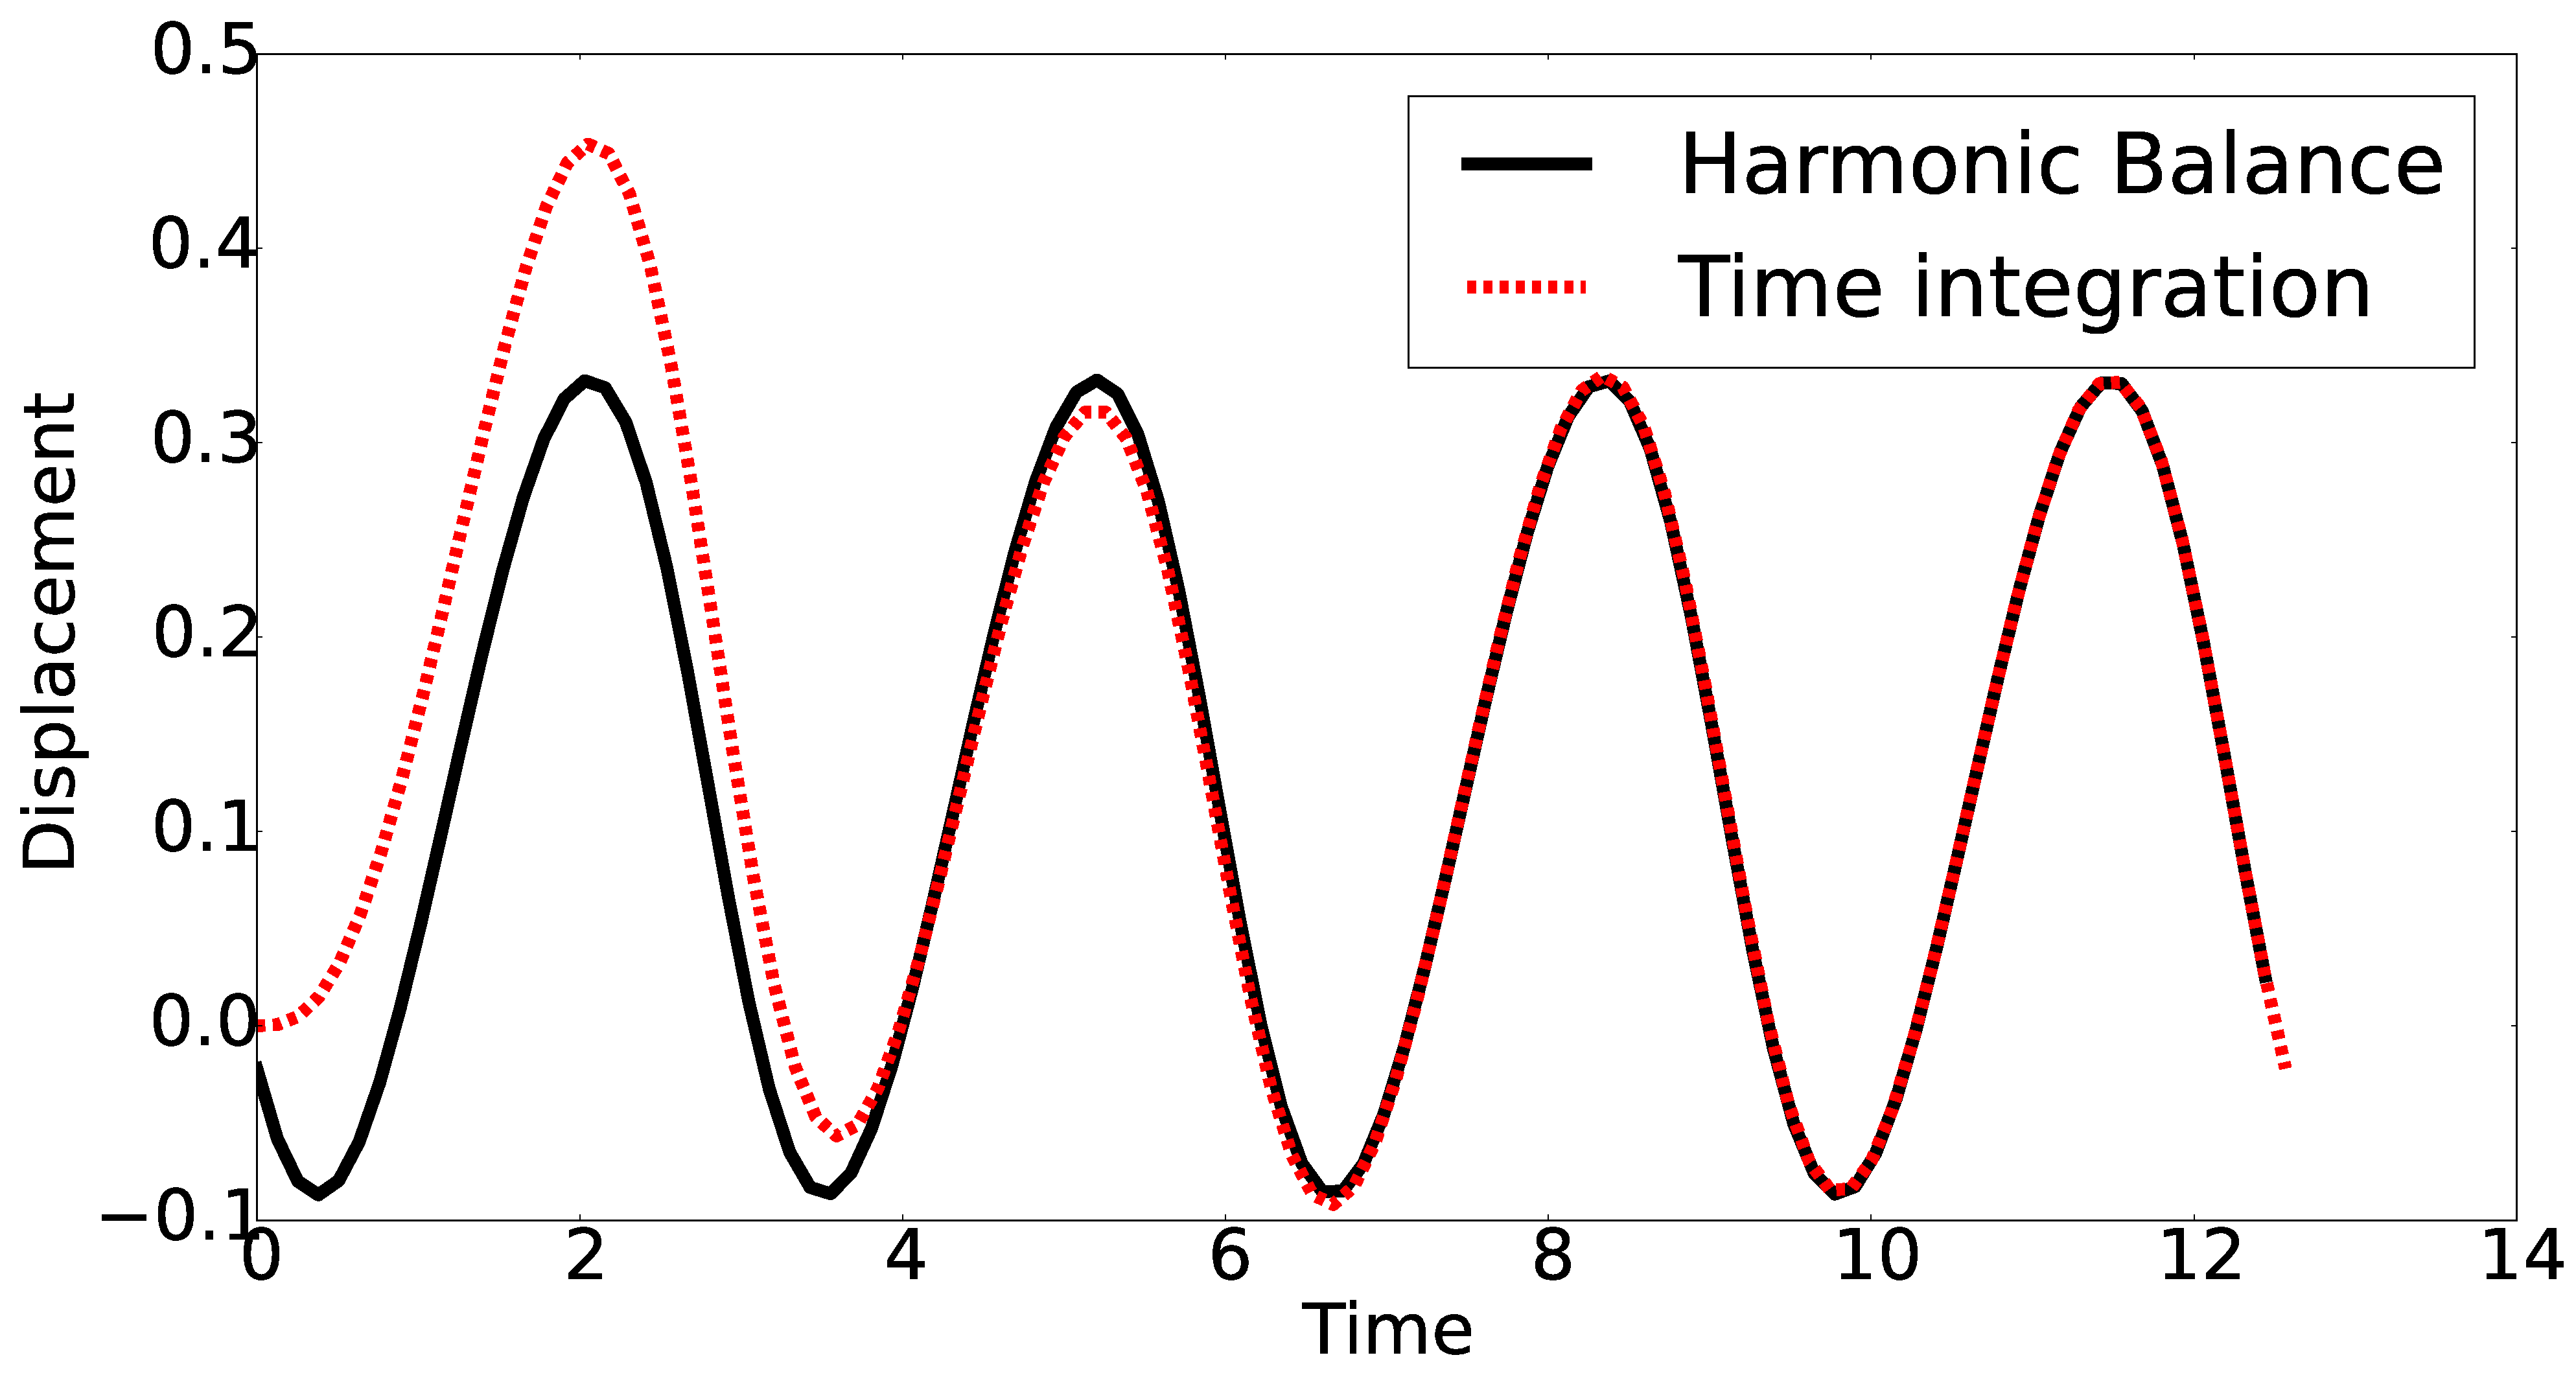
\includegraphics[width=8.0 cm]{figure/3N99.eps}
		\caption{n = 99}
    \end{subfigure}
    \caption{Comparison between HB and analytical result.}
    \label{fig:R3}
\end{figure}
% -------------------------------------------------------------------
\subsection{Double Pendulum}
Adapting Harmonic balance method for a two-degree of freedom system, a double pendulum, with $\theta_1$ and $\theta_2$ DOF is considered. If $m_1$, $m_2$, $l_1$ and $l_2$ are masses and lengths of pendulum 1 and pendulum 2 respectively, then the equations of motion are
\begin{equation}
(m_1+m_2) l_1 \ddot{\theta_1} + m_2 l_2 \ddot{\theta_2} \cos( \theta_1 - \theta_2 ) + m_2  l_2 \dot{ \theta_2 }^2 \sin( \theta_1 - \theta_2 )+g (m_1+m_2)  \sin( \theta_1) = 0
\end{equation}

\begin{equation}
m_2  l_2 \ddot{\theta_2}+m_2 l_1 \ddot{\theta_1} \cos(\theta_1 - \theta_2)-m_2  l_1 \dot{\theta_1}^2 \sin(\theta_1 - \theta_2)+m_2 g  \sin(\theta_2) = 0
\end{equation}


% -------------------------------------------------------------------
\subsection{Hypersonic Flutter}
The governing equation can be written as

\begin{equation}\label{eq:GE}
	m\ddot{\theta} + k \theta = f(\theta, t)
\end{equation}

where $m$ is the mass of airfoil, $k$ is the stiffness, $\theta$ is the angle of attack and $f$ is the aerodynamic load. We use the Piston Theory to calculate the aerodynamic load acting on the airfoil. We used the piston theory to calculate the pressure distribution on the airfoil \cite{ashley2012piston}.

\begin{equation}\label{eq:pistonTheory}
	\frac{P(x, t)}{P_\infty} = \left( 1+ \frac{\gamma - 1}{2} \frac{v_n}{a_\infty} \right)^{\frac{2 \gamma}{\gamma - 1}}
\end{equation}

where $P(x, t)$ is the pressure at point $x$ on the airfoil, $P_\infty$ is the free stream pressure, $\gamma$ is the ratio of specific heats and $a_\infty$ is the speed of sound. The third order expansion of Equation \eqref{eq:pistonTheory} results in

\begin{equation}
	P(x,t) = P_\infty
	\left[
	1 +
	\gamma \frac{v_n}{a_\infty} + 
	\frac{\gamma (\gamma + 1)}{4} \left( \frac{v_n}{a_\infty} \right)^2 + 
	\frac{\gamma (\gamma + 1)}{12} \left( \frac{v_n}{a_\infty} \right)^3
	\right]
\end{equation}

$v_n$ is calculated using the following equation.

\begin{equation}\label{eq:definitionOfVn}
	v_n = \frac{\partial Z(x,t)}{\partial t} + V \frac{\partial Z(x,t)}{\partial x}
\end{equation}

where $V$ is the free stream velocity and $Z(x,t)$ is the position of airfoil surface. The position of airfoil surface can be related to the angle of attack using the following equation:

\begin{equation}\label{eq:definitionOfZ}
	Z(x,t) = M_r\left( \theta(t) \right) Z_0(x)
\end{equation}

where $M_r$ is the rotation matrix, and $Z_0(x)$ is the initial shape of the airfoil.  As can be seen here, the location of surface at time $t$ only depends on the angle of attach at that time, $\theta(t)$. The rotation matrix is defined as

\begin{equation*}
	M_r = 
	\begin{bmatrix}
		\cos \theta & -\sin \theta \\
		\sin \theta & \cos \theta
	\end{bmatrix}
\end{equation*}

By expanding Equation \eqref{eq:pistonTheory}, and substituting for $Z(x,t)$ from Equation \eqref{eq:definitionOfZ}, Equation \eqref{eq:GE} can be rewritten as

\begin{subequations}
\begin{gather}
	m\ddot{\theta} + k \theta = 
	\oint_{airfoil} P_\infty
	\left[
	\gamma \frac{v_n}{a_\infty} +
	\frac{\gamma (\gamma + 1)}{4} \left( \frac{v_n}{a_\infty}\right)^2 +
	1
	\right] ds
	\\
	v_n = 
	\frac{\partial M_r(\theta)}{\partial t}Z_0(x) + V M_r(\theta)\frac{\partial Z_0(x)}{\partial x}
\end{gather}\label{eq:GEfull}
\end{subequations}

Equation \eqref{eq:GEfull} needs to be solved for $\theta$ using Harmonic Balance method. For this problem the operating conditions of the vehicle are selected as follows:

\begin{table}[htbp]
\begin{center}
\begin{tabular}{c|c}
	$\gamma$ & 1.4 \\ \hline
	$a_\infty$ & 343 m/s \\ \hline
	$P_\infty$ & 10 Pa \\ \hline
	V & 600 m/s \\
	\end{tabular}
	\end{center}
	\caption{Operating conditions.}
\end{table}

For verification, the harmonic balance results are compared with the numerical integration is Figure \eqref{fig:hypersonicFlutterResult}. As shown here, the harmonic balance predicts a static solution ($\theta(t_\infty) = -1.706$) however, the numerical integration predicts oscillation. The interesting point in here is that the time average value of numerical integration is the same as harmonic balance results. This means that the harmonic balance did not have enough frequency content to capture the oscillations. It only captured the constant term.

\begin{figure}[h]
	\centering
	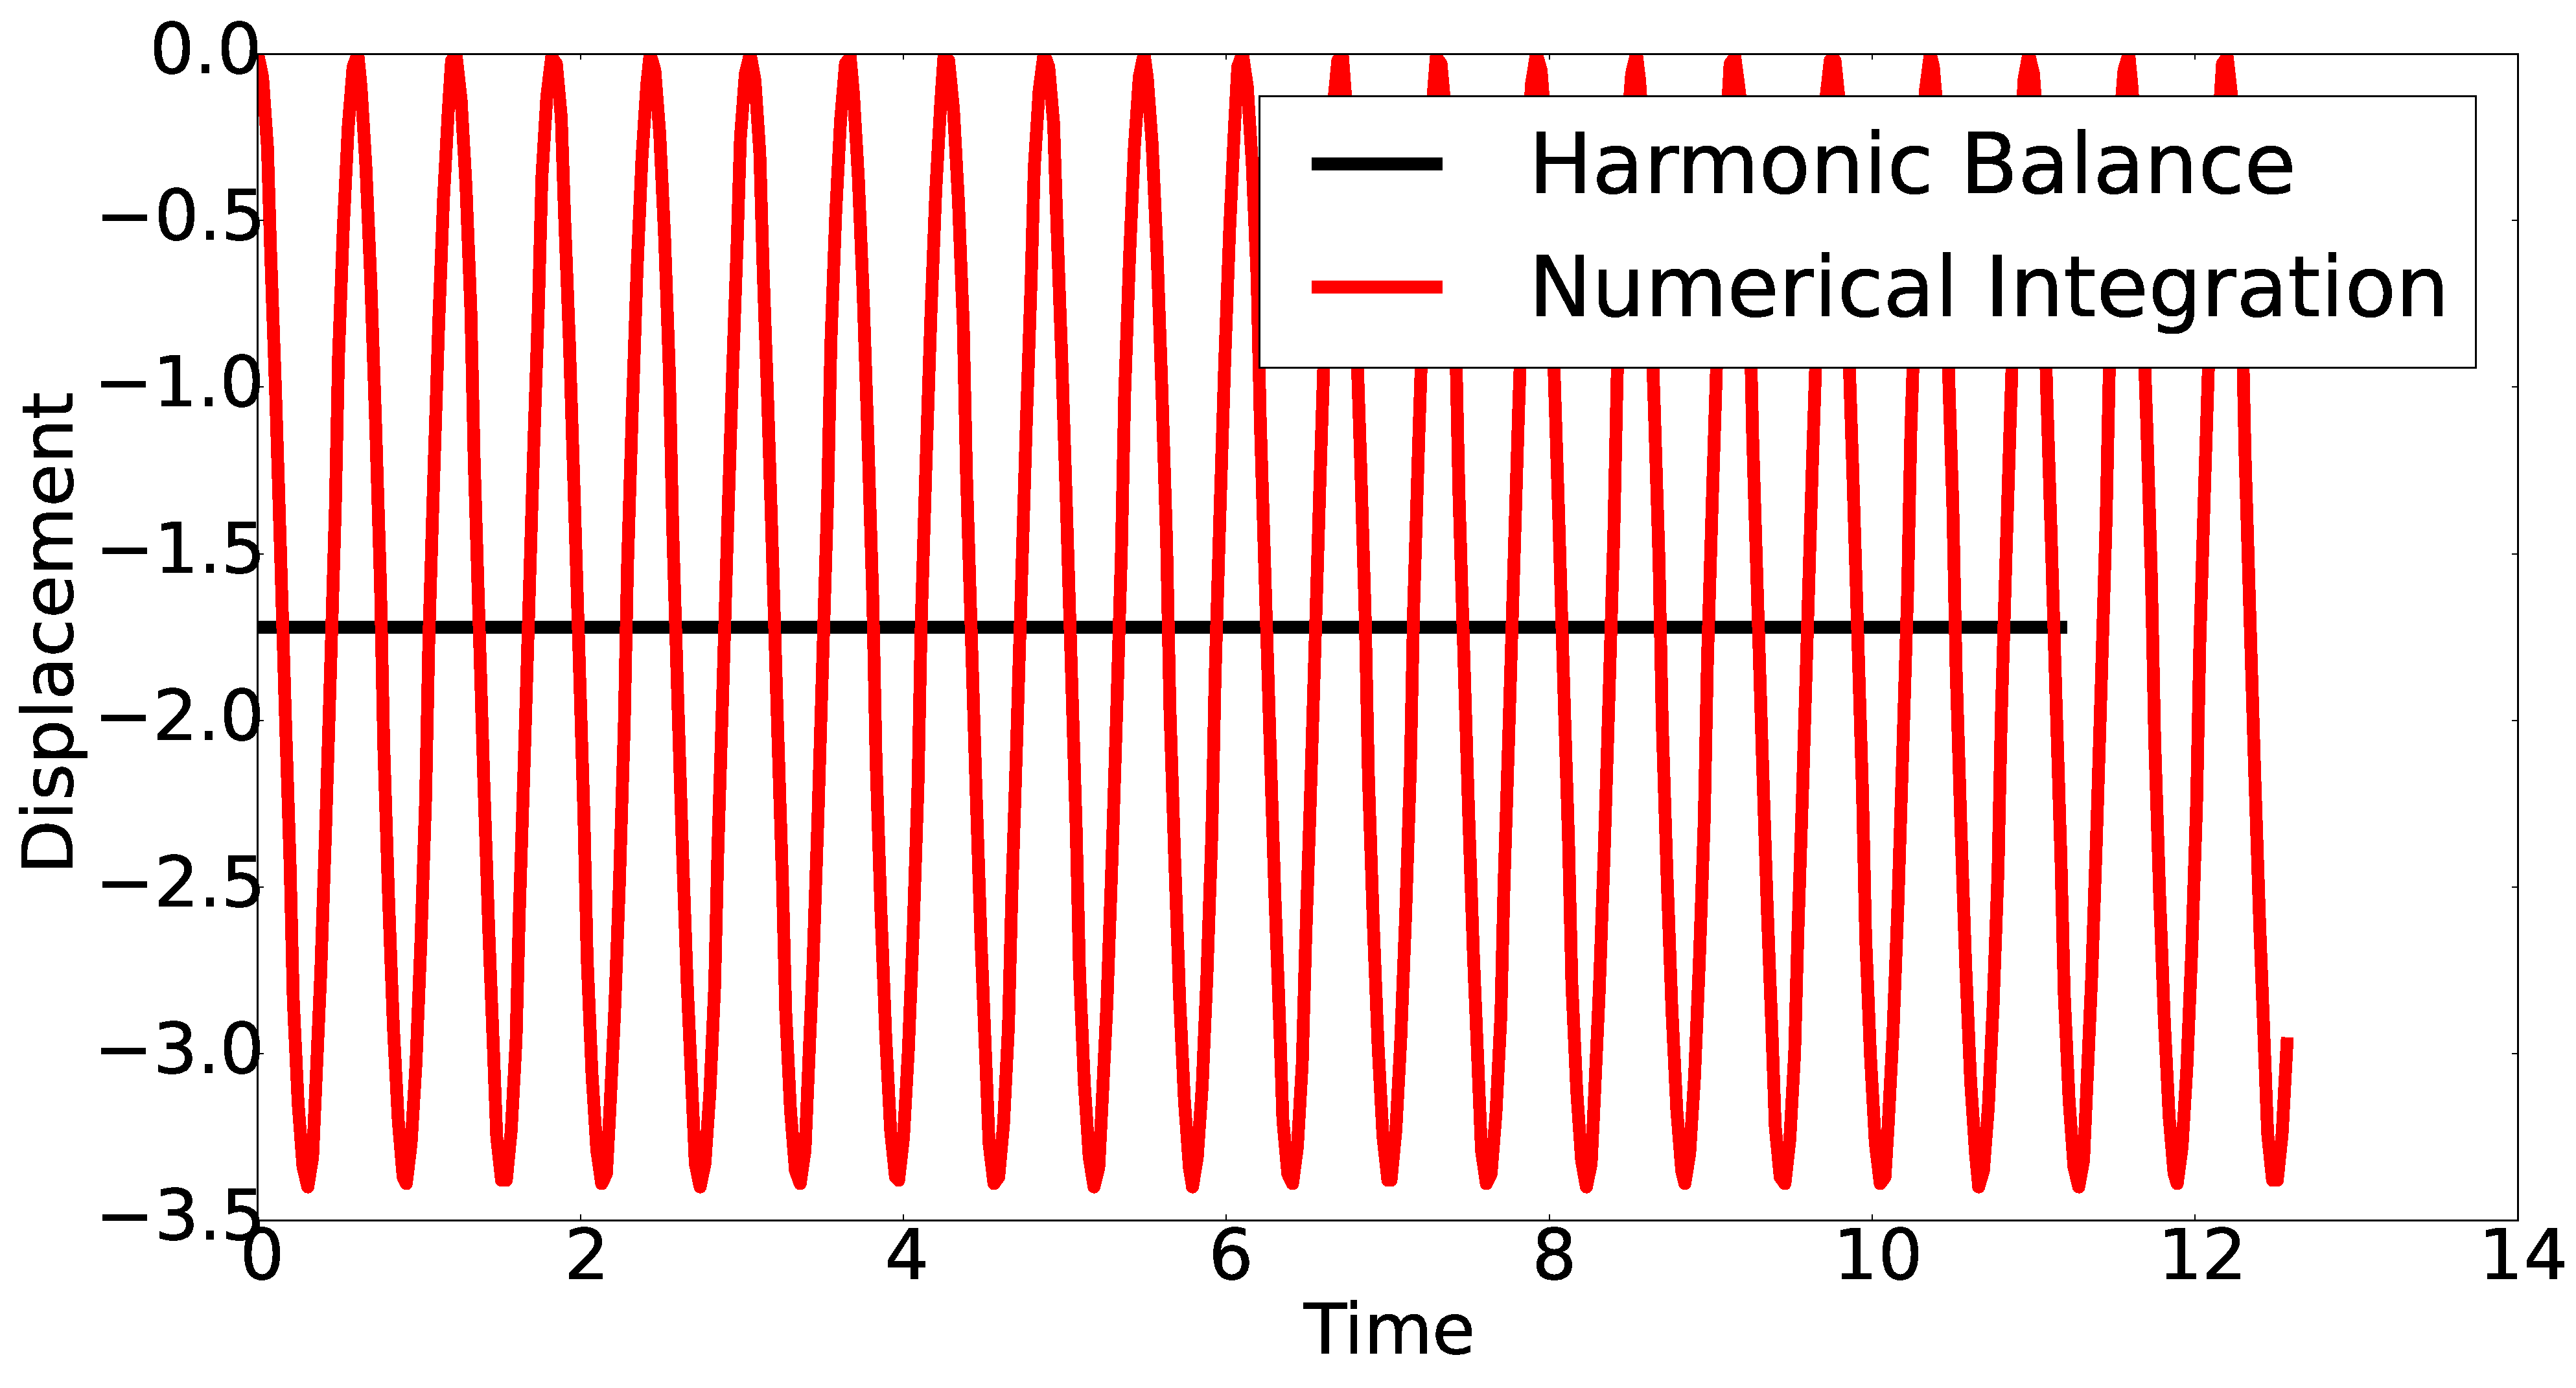
\includegraphics[width=12.0 cm]{figure/4N9.eps}
	\caption{Comparison between HB and analytical result}
	\label{fig:hypersonicFlutterResult}
\end{figure}

% ===================================================================
\bibliographystyle{aiaa}
\bibliography{ref}
\end{document}
